\ifnum\aluno=1
\renewcommand\chapterillustration{./abertura-combinatoria}
\else
\renewcommand\chapterillustration{./abertura-combinatoria-professor}
\fi


\renewcommand\chapterwhat{Problemas do cotidiano que envolvam o processo de contagem. Começando com a contagem de conjuntos de dados que podem ser enumerados e organizados em tabelas, árvores e/ou $n-$uplas, seguindo para a compreensão da necessidade do uso do  Princípio Multiplicativo e do Princípio Aditivo para solução de problemas combinatórios mais gerais.}
\renewcommand\chapterbecause{
Problemas de contagem estão presentes em várias situações do cotidiano, como por exemplo, a quantidade de senhas de um determinado padrão. Uma senha eficiente é aquela difícil de ser descoberta então quanto maior o número de senhas de um determinado padrão melhor se torna a segurança da senha criada. Outros exemplos são: quantidade de placas de automóveis; quantidade de dígitos em números de telefones; quantidade de jogos possíveis na loteria, quantidade de números de IP's (do inglês \textit{Internet Protocol}), escalas de trabalhos ou de aulas, etc. Combinados com o estudo de Probabilidade ajudam na tomada de decisão, ao ponto que fornecem as possibilidades de  ocorrência de determinados fatos. 

Problemas de contagem também estão presentes em outras áreas do conhecimento como Física, Biologia e Computação. Além disso, o raciocínio combinatório desenvolve características importantes na resolução de problemas de maneira geral como processos de reflexão e abstração, levantamento de hipóteses, escolha de caminho para a solução e construção de generalizações, processos de investigação, de construção de modelos, formulação e a testagem de conjecturas; enfim, resolução e elaboração de problemas recorrendo a estratégias diversas, habilidades gerais presentes na BNCC.} 
\chapter{Análise Combinatória}
\label{combinatoria-chap}

\mbox{}\thispagestyle{empty}\clearpage

\thispagestyle{empty}

\begin{center}
Projeto: LIVRO ABERTO DE MATEMÁTICA

\noindent \begin{tabular}{lcccr}

\includegraphics[scale=.15]{impa}& \quad\quad& 
\includegraphics[width=3cm]{logo} & \quad\quad& 
\includegraphics[scale=.24]{obmep} 
\end{tabular}
\end{center}

\vspace*{.3cm}

Cadastre-se como colaborador no site do projeto: \url{umlivroaberto.org}



% \begin{center}
%   \includegraphics[width=2cm]{canvas}
% \end{center}

\begin{tabular}{p{.15\textwidth}p{.7\textwidth}}
Título: & Análise Combinatória\\
\\
Ano/ Versão: & 2020 / versão 0.1 de \today\\
\\
Editora & Instituto Nacional de Matem\'atica Pura e Aplicada (IMPA-OS)\\
\\
Realização:& Olimp\'iada Brasileira de Matem\'atica das Escolas P\'ublicas (OBMEP)\\
\\
Produção:& Associação Livro Aberto\\
\\
Coordenação: & Fabio Simas, \\
			&  Augusto Teixeira (livroaberto@impa.br)\\
\\
  Autores: & Carlos A. Gomes (UFRN),\\
             & Lhaylla Crissaff (UFF).\\
        
\\
Colaboração: & \\
\\
Revisor: &  \\
         &  \\
\\
Design: & Andreza Moreira (Tangentes Design) \\
\\
  Ilustrações: & --- \\ 
\\
Gráficos: & ---\\
\\
  Capa: & Foto de James Sutton, no Unsplash \\
  		& https://unsplash.com/photos/qXn5L9BqRbE \\

\end{tabular}
\vspace{.5cm}



\begin{figure}[b]
\begin{minipage}[l]{5cm}
\centering

{\large Licença:}

  
\includegraphics[width=3.5cm]{cc-by-nc-sa}
\end{minipage}\hfill
\begin{minipage}[c]{5cm}
\centering
{\large Desenvolvido por}


\includegraphics[width=2.5cm]{logo-associacao.jpg}
\end{minipage}
\begin{minipage}[r]{5cm}
\centering

{\large Patrocínio:}
  \vspace{1em}
  
\includegraphics[width=3.5cm]{itau}
\end{minipage}
\end{figure}

\mainmatter





\explore{Princípios Fundamentais de Contagem}

Uma gincana está sendo organizada na escola. Para realização das atividades na gincana, a professora de uma turma com 40 estudantes quer organizar os grupos sorteando seus membros. Para isso possui 8 fitas de cada uma das seguintes cores: amarela, vermelha, laranja, branca e preta. Essas fitas serão escolhidas de maneria aleatória sendo misturadas em um recipiente que não seja possível verificar a cor da fita até que seja totalmente retirada.  Joana, uma aluna desta turma, tem um amigo muito querido e está torcendo para que fiquem no mesmo grupo. Será que as chances disso acontecer são grandes ou pequenas?


Para determinar se a chance de um evento ocorrer é grande ou pequena é preciso analisar a taxa de ocorrência deste evento. Em outras palavras, verificar se quantidade de possibilidades do evento ocorrer é grande ou pequena quanto comparada a quantidade total de eventos que podem acontecer. 
Contar o número de casos para responder a dúvida de Joana não é algo que possa ser feito construindo uma lista de todas as possibilidades. Isso levaria muito tempo! Vamos estudar aqui conceitos que ajudam nesta contagem, e em muitas outras, presentes no cotidiano. Esse conhecimento auxilia na tomada de decisões.  

Para caminharmos na direção da solução do problema proposto vamos primeiro desenvolver alguns conceitos de Análise Combinatória. 

\begin{task}{Escolhendo o nome da empresa}

\begin{figure}[H]
\centering

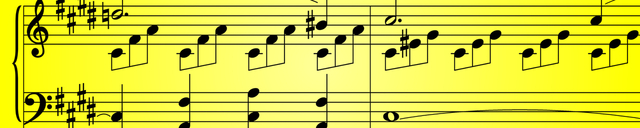
\includegraphics[width=.9\linewidth]{music.jpg}
\end{figure}

Três amigas, Mirella, Rayssa  e Isabela decidiram montar uma sociedade e gostariam que a empresa, do ramo da música, tivesse as inicias (primeira letra) de seus nomes.  

\begin{enumerate}

\item Quais seriam os possíveis nomes para a empresa? 

\item Depois de já terem pensado nas possibilidades de nomes, Letícia decidiu também fazer parte da sociedade. É preciso recomeçar a organização dos nomes ou é possível modificar os nomes já encontrados para que a letra L seja incluída? Quantos seriam agora os possíveis nomes?

\item Se as quatro iniciais tivessem sidos dadas inicialmente a estratégia de contagem teria sido a mesma utilizada no item b)?

\item Quantas seriam as distintas possibilidades usando 5 iniciais diferentes? E 6? E 7? Percebeu alguma regularidade? ( Fazer o caso com 2 letras pode ajudar a pensar na regularidade.)

\end{enumerate}

\end{task}

\begin{knowledge}
$n!$ (lê-se n fatorial) é uma simplificação para a expressão matemática $n!=n \cdot (n-1) \cdot (n-2) \cdots 2 \cdot 1.$ Esse símbolo aparece com muita frequência nos problemas de contagem. Por exemplo, para $n=2,$ $2!= 2 \cdot 1 = 2.$ Tomando agora $n=7,$ $7!=7 \cdot 6 \cdot 5 \cdot 4 \cdot 3\cdots 2 \cdot 1 = 5040.$ Observe que, apesar de $n$ ter crescido pouco, de $2$ para $7,$ o fatorial desses números tem um grande crescimento. A notação de exclamação foi introduzida por Christian Kramp, matemático francês, no trabalho \textit{ Éléments d'arithmétique universelle}. Veja mais em:

\begin{figure}[H]
\centering


\includegraphics[scale=0.45]{frame.png}   
\end{figure}
\end{knowledge}


\begin{task}{Nome da empresa com letras repetidas}


Três amigos, Marcos, Rayssa  e Roberto decidiram montar uma sociedade e gostariam que o nome da empresa, do ramo dos aplicativos, fosse formado pelas inicias (primeira letra) de seus nomes. 

Como seria pensar na quantidade de nomes da empresa se existissem nomes com mesmas iniciais ? Observando as soluções da Atividade \textbf{Escolhendo o nome da empresa} pense nas modificações necessárias para construir a solução deste novo problema.

\begin{enumerate}

    \item Quantos seriam os nomes possíveis se a sociedade tivesse apenas Rayssa e Roberto?
    \item Quantos seriam os possíveis nomes da empresa com os três amigos?
    \item Quantos seriam os nomes  possíveis para a empresa se Letícia decidisse participar da sociedade ?
    \item Quantos seriam os nomes possíveis se a sociedade tivesse quatro pessoas, das quais três possuem nomes com letras iniciais iguais e a outra pessoa letra inicial do nome diferente das demais?
    \item Quantos seriam os nomes possíveis se a sociedade tivesse quatro pessoas, duas a duas com letras iniciais iguais?
\end{enumerate}

\end{task}

\clearpage
\begin{knowledge}
As várias ordenações de letras de uma determinada palavra são chamadas de Anagramas. Seriam como palavas, não necessariamente com sentido, que podem ser formadas a partir de um dado conjunto de letras. Saiba mais sobre a história e curiosidades dos Anagramas em 
\begin{figure}[H]
\centering


\includegraphics[scale=0.45]{frame3.png} 
\end{figure}
\end{knowledge}

\begin{task}{Jogo de dominó}
\textit{Inspirada em \url{ https://olimpiada.ic.unicamp.br/static/extras/obi2019/provas/ProvaOBI2019_f1p1.pdf} }

\begin{figure}[H]
\centering

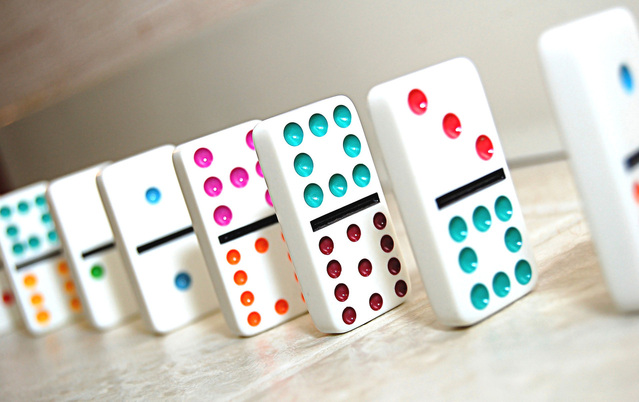
\includegraphics[scale=1]{domino.jpg}
\end{figure}


%{https://pt.freeimages.com/photo/domino-effect-4-1170138}
Em um jogo de dominó cada jogador começa com 7 peças, caso sobrem algumas, estas ficam para serem compradas durante a partida. As peças, todas distintas, são compostas por duas partes, cada uma das partes apresentando pontos que variam de 0 até 6, sendo permitido que a peça tenha duas partes iguais.
 
\begin{enumerate}

\item Escolha um critério de organização das peças de um dominó. Explique aos colegas o motivo dessa escolha.

\item Quantas peças tem um dominó convencional? Qual é o número máximo de jogadores por partida?

\item Imaginando um jogo de dominó com o número de pontos variando de 0 até n em cada parte. Qual o menor número n para que 5 pessoas possam jogar, iniciando com 7 peças cada?

\item Como encontrar o número de peças de um dominó com peças que permitam até 8 pontos em cada um de seus dois lados? 

\item Como saber a quantidade de peças de um dominó que tenha até $n$ pontos em cada um de seus lados?

\end{enumerate}

\end{task}

\begin{knowledge}
Saber se a ordem de organização dos elementos de um agrupamento influencia na contagem é muito importante. Perceba que para o nome da empresa a ordem em que as letras aparecem na palavra muda o nome criado, já para o conjunto de dominós a organização das peças é indiferente para o número total de peças. 
\end{knowledge}

\begin{task}{Desfios da coloração de mapas}
\label{coloracao-mapas}

Alguns desafios de contagem aparecem em redes sociais. O mais atrativo neles é que parecem simples, mas quando percebemos já perdemos horas tentando e não chegamos a solução correta. Quem é que não gosta de um bom desafio, não é?! 
Vejam esse simples mapa abaixo. 

\begin{center}
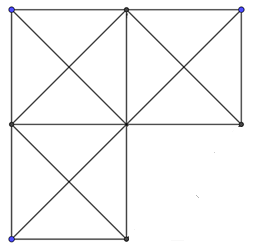
\includegraphics[scale=0.7]{triangulos.png}
\end{center}

\begin{enumerate}
\item Quantos triângulos o mapa possui? Como realizou a contagem?
\item Use duas cores para pintar os triângulos menores de modo que aqueles que tiverem lados em comum não sejam coloridos com a mesma cor. 
\item Compare sua pintura com a do seu colega.  De quantas maneiras distintas foi possível colorir o mapa? 
\item Foi possível perceber alguma característica nas colorações do item b)?
\item Dispondo de três cores, utilize todas para pintar os triângulos menores de modo que aqueles que tiverem lados em comum não sejam coloridos com a mesma cor.
\item Qual foi a estratégia que você utilizou para chegar nessa configuração de cores?
\item Quantas configurações diferentes de cores apareceram na turma?
\item Como podemos contar todas as configurações possíveis?
\item Será que existe um mapa que não possa ser colorido com menos de $4$ cores, seguindo a restrição de que regiões que possuem fronteiras não sejam coloridas coma a mesma cor? Tente encontrar um exemplo. Se ele existe que característica precisa ter? Se não existe, por qual motivo não existe?
\end{enumerate}

\end{task}

\begin{knowledge}
Quatro cores são suficientes para colorir qualquer mapa de modo que regiões fronteiriças (que possuem um lado em comum) não sejam pintadas da mesma cor.  Este problema esta intimamente ligado a Teoria dos Grafos. Saiba mais em:  
%https://teses.usp.br/teses/disponiveis/55/55136/tde-26112016-112047/publico/CarlosLaercioGomesdeLima_revisada.pdf

\begin{figure}[H]
\centering

    
\includegraphics[scale=0.45]{frame (1).png}
\end{figure}


Na Atividade \hyperref[coloracao-mapas]{Desafios da coloração de mapas} você deve ter se perguntado sobre a importância de pensar no número de colorações de um determinado mapa. Esta atividade poderia estar modelando o seguinte problema: Uma escola técnica possui 12 disciplinas e precisa organizar seus horários de exame final tomando o cuidado para que o aluno não tenha que realizar dois exames no mesmo período. As 12 disciplinas poderiam ser associadas aos triângulos pequenos e as fronteiras representariam as disciplinas que possuam alunos em comum para a realização da prova. As provas podem ser organizadas usando apenas dois períodos? Isso pode ser feito de quantas maneiras diferentes? Usando três períodos, quantas são as possibilidades de organização?
Segue também QR Code para o Jogo das Quatro Cores

\begin{figure}[H]
\centering

    
\includegraphics[scale=0.4]{frame4.png}
\end{figure}

%\url{http://www.matematica.seed.pr.gov.br/modules/conteudo/conteudo.php?conteudo=366} 
que consiste em colorir um mapa usando no máximo $4$ cores com as mesmas restrições descritas anteriormente.
\end{knowledge}

\arrange{Princípios Fundamentais de Contagem}

Os problemas estudados em Análise Combinatória são aqueles que se preocupam em contar a quantidade de agrupamentos com determinadas condições. O objetivo é contar todas as variações possíveis sem ter que listar as possibilidades, é quantificar sem necessariamente visualizar. Quando a tarefa é pequena mostrar todos os resultados pode até ser simples e útil, mas no geral as soluções logo se tornam trabalhosas demais. As duas ferramentas descritas aqui resolvem a grande parte dos problemas de contagem.

Para compreender o \textbf{Princípio Multiplicativo} vamos considerar dois questionamentos: De quantas maneiras um grupo pode escolher um(a) capitão(ã) e um(a) vice capitão(ã)? De quantas maneiras um grupo pode escolher dois membros para participar de um jogo de cartas? Vamos considerar aqui o grupo com 8 integrantes que a professora formou lá no início do livro. 

As duas perguntas parecem iguais, mas para o jogo de cartas não faz diferença quem foi o primeiro membro escolhido e quem foi o segundo, importa somente que dois sejam escolhidos. Mas quando se trata de capitão(ã) e vice essa escolha é diferente, pois capitã Júlia e vice Marcos é diferente de capitão Marcos e vice Júlia. 

Para simplificar vamos chamar os membros da equipe de 
$$M_1, M_2, M_3, M_4, M_5, M_6, M_7, M_8.$$

Observe a árvore de possibilidades: 


\begin{figure}[H]
\centering

    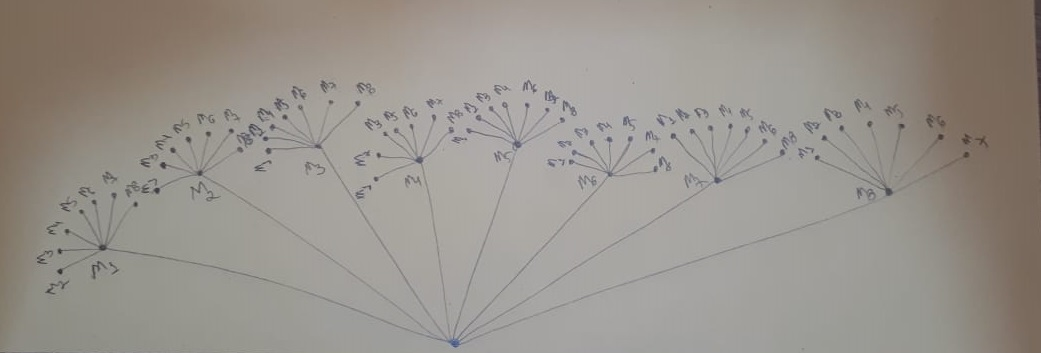
\includegraphics[scale=0.5]{arvore1.jpg}
\end{figure}


Saindo da raiz da árvore existem 8 possibilidades $\{M_1, M_2, M_3, M_4, M_5, M_6, M_7, M_8\}$ para a escolha do primeiro membro. Depois o segundo ramo da árvore, contem as possibilidades que estão disponíveis, após a primeira escolha. Qualquer membro que for escolhido para capitão(ã) tem disponível 7 membros para ser vice, as possibilidades são diferentes, mas as quantidades não. Para encontrar o total podemos somar oito parcelas iguais a 7, cada uma correspondendo a contagem feita tomando como referência um membro da equipe, correspondendo a um ramo da árvore. Este cálculo pode ser simplificado como oito vezes sete :

$$7+7+7+7+7+7+7+7=  8 \cdot 7= 56.$$

De maneira resumida, deve ser realizada a multiplicação do número de possibilidades de escolha do(a) capitão(ã)  pelo número de possibilidades de escolhas do(a) vice. O importante é perceber que nesta contagem $M_1M_2  \neq M_2M_1$, pois nas 8 possibilidades iniciais foram considerados todos os membros, ou seja, tanto $M_1$ quanto $M_2$.  

Ao escolher um representante para ser o(a) capitão(ã), os(as) possíveis vices mudam, mas o número de possibilidades não muda. Por isso o \textbf{Princípio Multiplicativo} pode ser usado, pois se refere a uma soma de parcelas iguais. Mas neste caso como a contagem está sendo feita sempre do mesmo conjunto de dados, a utilização deste princípio leva em conta a ordem dos elementos.

De maneira geral,  se para cada ocorrência de um determinado fato o número de ocorrências de outro fato não se altera, então o número de ocorrências dos dois fatos juntos, ou de maneira sucessiva,  é dado pelo produto das possíveis ocorrências de cada um, é o que garante o \textbf{Princípio Multiplicativo}. 

Este princípio pode ser utilizado em muitos contextos e repetidas vezes. Imagine que a escolha fosse relativa a capitão(ã), vice e um(a) substituto(a). Seriam três posições para serem ocupadas, oito possibilidades para a primeira, sete para a segunda e seis para a terceira. Cada escolha feita para capitão(ã) e vice deixa disponível seis possibilidades de escolha para o(a) substituto(a), logo seriam $8\cdot 7 \cdot 6$ possibilidades de escolha.

Para a construção das duplas na pergunta do jogo de cartas a ordem não é importante, a dupla $M_1M_2 = M_2M_1 = \{M_1,M_{2}\}$. Isso quer dizer que a cada uma das soluções procuradas será contabilizada duas vezes se o \textbf{Princípio Multiplicativo} for utilizado. São duas cópias da mesma solução. por isso a solução procurada é dada por $\dfrac{8 \cdot 7}{2}$.

 Se a ideia fosse escolher trios, da mesma forma seriam $8\cdot 7 \cdot 6$ maneiras de escolher 3 pessoas com ordem de escolha. Pegando uma sequência de três pessoas, digamos $M_1M_2M_3$, elas podem ser organizadas de 6 maneiras diferentes em fila (que corresponde ao número total de trocas de posições dadas entre elas, calculada por 3!=6), mas quando o interesse é por trios, essas seis variações representam o mesmo trio: $M_1M_2M_3=M_1M_3M_2=M_2M_1M_3=M_2M_3M_1=M_3M_1M_2=M_3M_2M_1=\{M_1,M_{2},M_{3}\}.$
 
 Como isso  ocorre para quaisquer três membros diferentes, cada solução procurada foi contabilizada seis vezes, foram contadas seis cópias da mesma solução, e para retirar a repetição é preciso fazer a divisão por $3!=6$, $$\dfrac{8 \cdot 7 \cdot 6}{6} = 8 \cdot 7 = 56.$$

O \textbf{Princípio Multiplicativo} impõe uma ordem quando os elementos são tomados no mesmo conjunto e a divisão deve ser usada quando é preciso retirar a ordem da contagem. Mas se o agrupamento é formado com elementos de conjuntos disjuntos (que não têm elementos em comum) o \textbf{Princípio Multiplicativo} não impõe ordem. Se a ordem for desejada depois de encontrada a solução, deve-se levar em conta as permutações possíveis dos elementos de uma dada solução. 

Para ficar mais claro, considere que será preciso escolher uma dupla de juízes para uma das atividade em sala, sendo um do grupo $G_1=\{G_{11},G_{12},G_{13},$
$G_{14},G_{15},G_{16},G_{17},G_{18}\}$ e um do grupo $G_2=\{G_{21},G_{22},G_{23},
G_{24},G_{25},G_{26},$ $G_{27},G_{28}\}$. Existem 8 possibilidades para a escolha dos membros de cada grupo:


\begin{figure}[H]
\centering


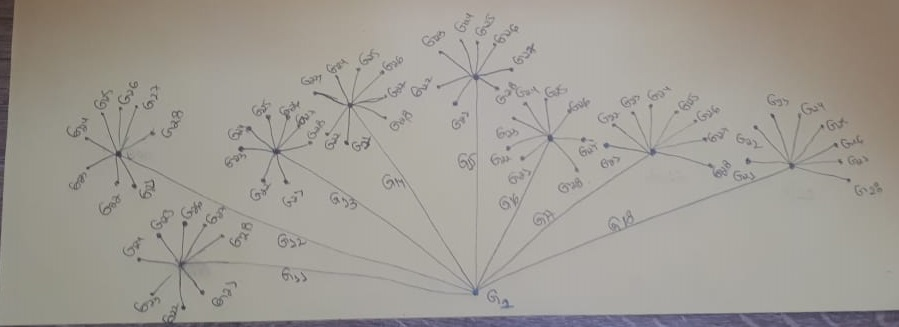
\includegraphics[scale=0.5]{arvore2.jpg}
\caption{$G_{ij}$ indica o membro $j$ do grupo $i$.}
\end{figure}

 $$8+8+8+8+8+8+8+8=  8 \cdot 8.$$
 
Mas neste caso só faz sentido considerar $G_{21}G_{11}$, quando a contagem for organizada a partir do grupo $G_2$, pois $G_{21}$ não faz parte do grupo $G_1$. Para este problema, apesar da escolha estar sendo feita para duplas, não existe a necessidade da divisão por 2, pois não existem cópias da mesma solução. Cada membro foi escolhido de um grupo diferente de possibilidades. Tendo escolhido qualquer membro de $G_1$ restam sempre as mesmas possibilidades para a escolha do membro de $G_2$, que são todos os membros do grupo. Caso seja necessário impor ordem nesta contagem é preciso multiplicar pelas variações possíveis, que seria o mesmo que usar o \textbf{Princípio Aditivo}.

O \textbf{Princípio Aditivo}, diz que se um problema de contagem puder ser separado em problemas menores que não possuam casos em comum, a solução para o problema mais geral pode ser calculada como a soma das soluções dos problemas menores que o compõe. 

Ao dizer que os problemas menores não possuem soluções comuns, a solução geral está sendo construída como soma de soluções que fazem parte de conjuntos disjuntos (conjuntos separados). 

O raciocínio feito para se chegar ao \textbf{Princípio Multiplicativo}  usa do \textbf{Princípio   Aditivo},  pois a solução foi construída como a soma de várias soluções menores. No geral, o \textbf{Princípio Aditivo} aparece em problemas que possuem restrições que devem ser consideradas separadamente. 

Considere que na formação dos juízes duas pessoas não poderiam estar juntas, isso gera restrições na contagem, a solução pode ser dada como a soma de três casos: duplas formadas com  $P_1$ e sem $P_2$; duplas formadas com  $P_2$ e sem $P_1$ e as duplas formadas sem $P_1$ e sem $P_2$. Outra maneira de resolver este mesmo problema é com o uso da subtração. Assim como a divisão é usada para retirar as cópias da solução a subtração é usada para retirar algumas soluções contabilizadas a mais. Neste último problema, a contagem poderia ter sido feita considerando todas as duplas possíveis e depois retirada dela as duplas com $P_1$ e $P_2$ juntas. 

\practice{Princípios Fundamentais da Contagem}

\begin{task}{Jogo da senha}

\begin{figure}[H]
\centering

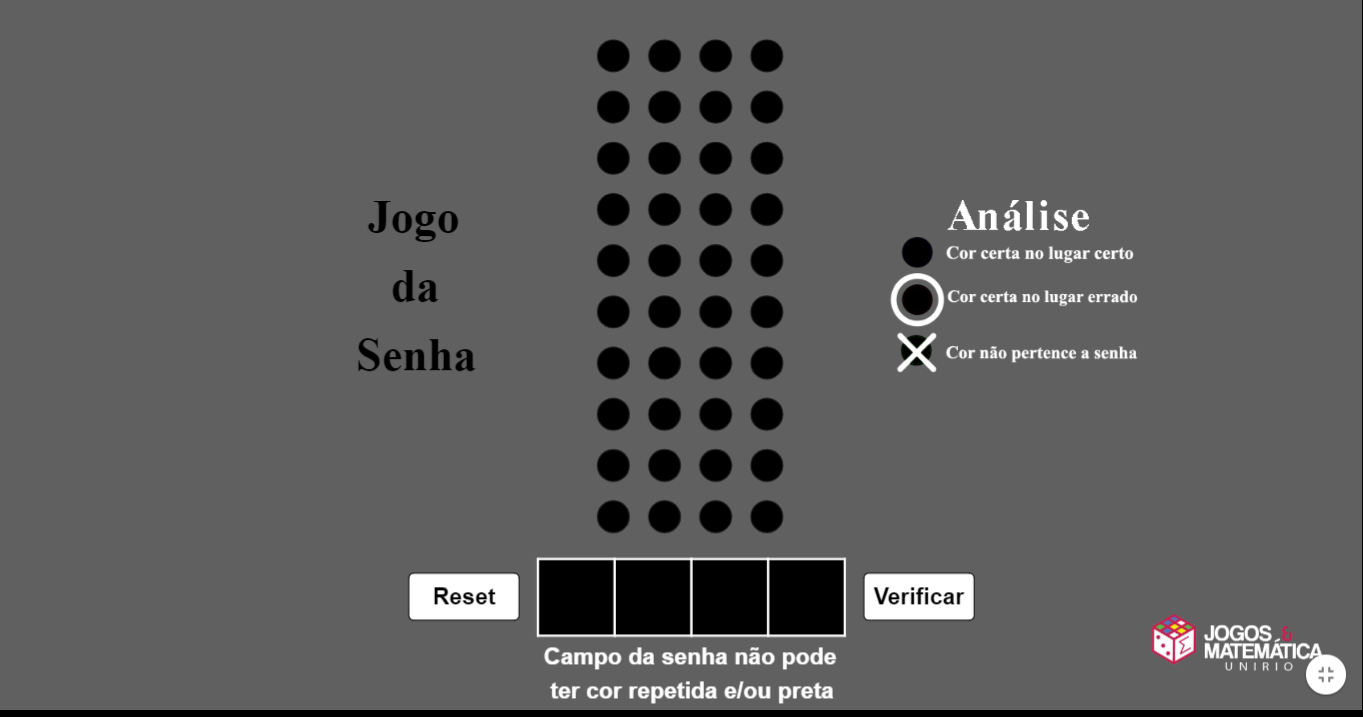
\includegraphics[scale=0.3]{jogosenha.png}
\end{figure}

A senha é composta por 4 cores distintas. Clique em cada um dos 4 quadrados para selecionar uma cor dentre seis disponíveis, e em seguida clique no botão verificar. Sua tentativa será salva nas linhas com 4 bolinhas, e automaticamente é gerado uma análise como pode ser conferida na tela do jogo. O jogador deverá observar análise feita antes de seguir para a próxima tentativa. Vence o jogador que acertar a senha com o menor número de tentativas.



Clique para jogar: \url{https://www.geogebra.org/m/rjyuwp2j}.



Referência: ( Este jogo faz parte de um projeto
\url{https://jogosmatunirio.wordpress.com/jogos-digitais/}) 



Depois de jogar discuta com seus colegas as questões abaixo. 

\begin{enumerate}

\item Qual foi o maior número de tentativas feitas na turma para acertar a senha? 
\item Seguindo todas as dicas, é possível saber qual seria o número máximo de tentativas para acertar a senha? Se sim, determine esse número.
\item Quantas senhas é possível formar neste jogo?
\item Caso o jogo não fornecesse as dicas qual seria o número máximo de tentativas para acertar a senha?
\item Quantas senhas seriam possíveis de ser formadas se as cores fossem trocadas por 6 números ou 6 símbolos sem que seja permitida a repetição?
\item Qual seria o número de senhas possíveis se fosse permitido repetir as cores?
\item Qual seria o número de senhas possíveis se fossem usadas 2 cores distintas e 2 números distintos, de um total de 6 cores e 10 números de modo que as cores fiquem juntas e os números também?
\item Levando em conta que quanto mais possibilidades de senhas mais segurança para os usuários, já que descobrir a senha por tentativas se torna uma tarefa difícil, seria melhor uma senha que permitisse ou não repetição de caracteres?

\item Dada uma senha do tipo dado no exercício, quais modificações poderiam ser feitas em sua construção para tornar mais difícil de determiná-la ?

\item A ordem em que as cores aparecem muda a senha representada. Crie um problema de contagem onde a ordem da escolha não impacta na solução do problema.
\end{enumerate}


\end{task}


\explore{Contando Agrupamentos}

O número de maneiras de se retirar 3 bolas amarelas e 2 vermelhas de uma urna com 5 bolas, sem reposição, tem alguma relação com o número de maneiras de se escolher 3 pessoas de um grupo de 5? Será que problemas completamente diferentes podem ter a mesma solução?

\begin{task}{Sistema Braille}

\textit{Esta atividade está baseada no texto: 
 \url{http://www.ibc.gov.br/images/conteudo/DPPE/Geral_departamento/2019/colecaoapostilas/Simbologia-Braille_2019_public.pdf} Todas as imagens forma retiradas desta bibliografia.}
 
 
 
 
 A atividade foi pensada para ser relacionada o material de Pensamento Computacional.
 
 
 
 Criado por Louis Braille, braille é um sistema de escrita e leitura tátil. Ele é determinado por um arranjo de seis pontos em relevo, dispostos em três linhas, com dois pontos em cada linha. O conjunto desses seis pontos é também conhecido como \textit{cela braille} ou \textit{célula braille}, com ilustração dada por  

\begin{figure}[H]
\centering

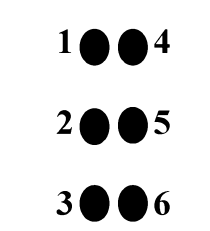
\includegraphics[scale=0.4]{braille2.png}
\end{figure}

Os pontos da célula braille são numerados na seguinte forma:

\begin{itemize}
    \item coluna da esquerda (do alto para baixo) pontos 1, 2 e 3;
    \item coluna da direita (do alto para baixo) pontos 4, 5 e 6.
\end{itemize}
A ordem Braille é uma organização dos símbolos em 7 séries.
\begin{itemize}
    \item A primeira série é denominada série superior constituída pelo símbolo contendo somente o ponto 1; por todos os símbolos que possuem o ponto 1 e são gerados utilizando pontos dentre 2, 4 e 5; o símbolo gerado pelos pontos 2 e 4; e o símbolo gerado pelos pontos 2, 4 e 5.
    \item A segunda série é construída acrescentando o ponto 3 a cada símbolo da primeira série;
    \item A terceira série resulta da adição dos pontos 3 e 6 a cada símbolo da primeira série;
    \item A quarta série é construída com a inclusão do ponto 6 a cada símbolo da primeira série;
    \item A quinta série é denominada série inferior constituída pelo símbolo contendo somente o ponto 2; por todos os símbolos que possuem o ponto 2 e são gerados utilizando pontos dentre 3, 5 e 6; o símbolo gerado pelos pontos 3 e 5; e o símbolo gerado pelos pontos 3,5 e 6.
    \item A sexta série possui como elementos a célula Braille contendo somente o ponto 3; os símbolos contendo o ponto 3 e gerados utilizando pontos dentre 4, 5 e 6; não contados anteriormente na quinta série.
    \item A sétima série é formada pelas sinais gerados somente pelos pontos da coluna direita, ou ainda, todas as células geradas utilizando pontos dentre 4, 5 e $6.$
    
\end{itemize}

\begin{figure}[H]
\centering

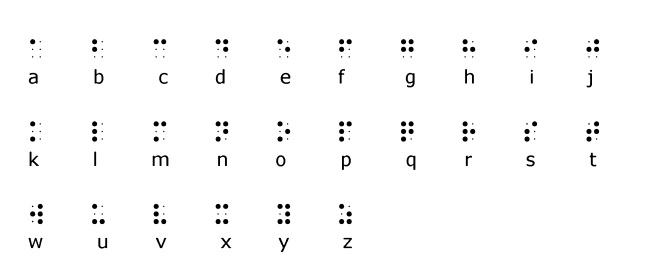
\includegraphics[scale=0.5]{alfabeto.jpg}
\caption{Alfabeto Braille}
\end{figure}

 
 
 \begin{enumerate}
     \item As diferentes disposições dos pontos na célula Braille permitem a formação de quantos símbolos braille?
     \item Quantos elementos possui a primeira série?
     \item Quantos elementos possui a sexta série?
     \item Quantos elementos possui a sétima série?
     \item Quantos símbolos é possível fazer com 1 ponto? Com 2 pontos? Com 3 pontos? Com 4 pontos? Com 5 pontos? Com 6 pontos? Somando todas estas possibilidades qual o valor encontrado?
      \item Olhando, por exemplo, para o teclado de um computador é possível representar todas as teclas por algum símbolo descrito no item a)? 
     
 \end{enumerate}

\end{task}

\begin{knowledge}
A técnica empregada no item \titem{d)} desta atividade, fazer a contagem por dois caminhos distintos e com isso concluir que expressões são iguais, é chamada de demonstração combinatória e é muito utilizada na matemática discreta. Algumas demonstrações que levariam muito tempo para serem feitas algebricamente são demostradas rapidamente por argumentos combinatórios. Veja o vídeo \textit{ PAPMEM - Janeiro de 2020 - Como mexer com coeficientes binomiais sem sujar as mãos}: \url{https://www.youtube.com/watch?v=69HLi6kG_us} para conhecer algumas demonstrações.
\end{knowledge}

\begin{task}{Indo de um ponto a outro}

Com um mapa abaixo, suponha que você está no ponto $A$ e precise chegar ao ponto $B.$ 

\begin{figure}[H]
\centering

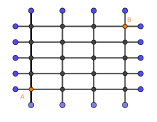
\includegraphics[scale=1.3]{caca_tesouro.png}
\end{figure}

\begin{enumerate}
\item Trace um possível caminho de $A$ até $B$ sendo possível somente andar nas  direções direita e para cima.
\item Compare os caminhos com os do colega de grupo, depois da turma. Tiveram muitos caminhos distintos?
\item Escolha um dos caminhos e dê instruções para um outro amigo da turma, explicando como chegar. 
\item Se todos os quarteirões têm a mesma medida, os caminhos da turma tiveram comprimentos iguais ou diferentes?
\item Seguindo as restrições do problema, qual o número de diferentes caminhos existentes entre você e o ponto $B?$ 

\end{enumerate} 

\end{task}

\begin{task}{Jogo da Mega-Sena}
Passando pelo site do Banco Caixa Econômica Federal é possível encontrar a seguinte tabela de probabilidades. A probabilidade aqui está definida como uma taxa, que representa a chance de ganhar o prêmio, calculada como a divisão entre o número de casos favoráveis e o total de possibilidades de sorteios do prêmio.  
  

\begin{figure}[H]
\centering

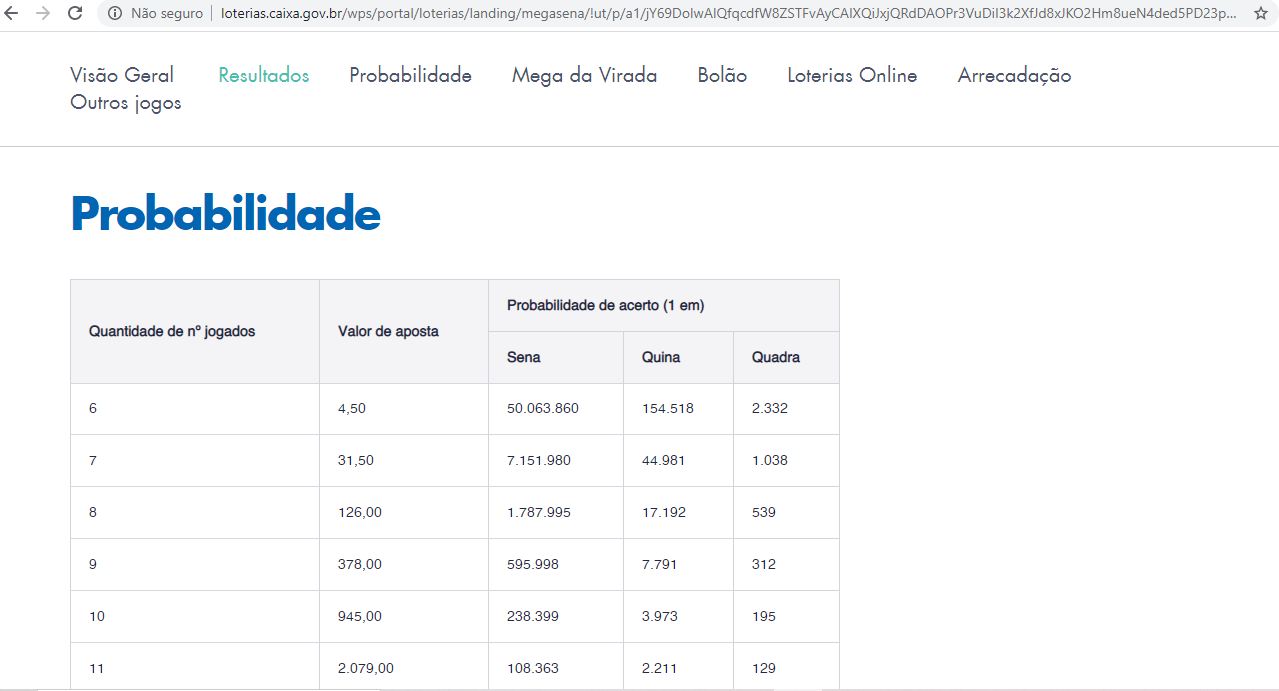
\includegraphics[width=\linewidth]{caixa_c.png}
\end{figure}


Sabendo que o jogo é feito com a escolha de pelo menos 6 números dentre as possibilidades de 1 até 60. Responda:

 \begin{enumerate}
     \item Como calcular a probabilidade de ganhar o prêmio da Sena ( acertar os seis números), Quina (acertar 5 números) e Quadra (acertar 4 números) com um jogo de 6 números?
     \item Para fazer o jogo com 6 números pago $R\$4,50$. Por qual motivo a escolha de sete números me custa  $R\$31,50$?
     \item E como recalcular as probabilidades para os prêmio da Sena, Quina e Quadra com 7 números?
     \item Fazendo 7 jogos de 6 números tenho maior probabilidade de ganhar do que fazendo 1 jogo de 7 números?
     \item A estimativa de prêmio do próximo jogo da Sena é de $R\$ 6$ milhões. Para fazer o jogo com 6 números pago $R\$4,50,$ quanto eu tenho que dispor de dinheiro para jogar todas as possibilidades do sorteio ? Valeria a pena jogar todos as combinações possíveis? Senão, supondo que somente pudesse ganhar sozinho, quanto deveria ser o prêmio para que valesse a pena fazer todas as apostas possíveis para a Sena ?
\end{enumerate}
\end{task}
\clearpage

\begin{task}{Alocando-se no cinema}
Um grupo de 12 amigos chegaram bem tarde para assistir um filme no cinema, não sendo possível encontrar todos os lugares juntos. Havia 8 lugares na parte da frente e 4 lugares na parte de trás da sala de cinema. Levando em conta que 2 deles não gostam da ideia de sentar-se no fundo e 3 deles não gostam da ideia de sentar-se na frente. Gabrielly decidiu então organizar a galera, visto que não foi permitido que se sentassem no corredor. Certeza que optariam por esse caminho! Observe a sequência de decisões (ações) que ela tomou:

\begin{itemize}
\item $A_1:$ Alocou os 3 que não gostam de 
sentar-se na frente, nas poltronas do fundo;

\item $A_2:$ Colocou no lugar que sobrou na parte de trás uma amigo que é indiferente ao lugar;

\item $A_3:$ Na frente colocou os outros amigos que faltavam. 
\end{itemize}


\begin{enumerate}
\item Acredita que a estratégia de organização foi eficaz? Por quê?
\item Existe outra maneira de organizar os amigos sem ferir as preferências?
\item Seria possível começar a organizar os amigos por aqueles que são indiferentes ao lugar? 
\item Pedro não gostou da organização pensada, mas diante das inúmeras possibilidades de organização do grupo desistiu de tentar. São mesmo muitas maneiras distintas de organização se as poltronas são numeradas? Como fazer para contar todas?
\end{enumerate}
\end{task}

\begin{task}{Analisando a solução do colega}
O seguinte exercício foi apresentado pela professora para uma turma que estava estudando Análise Combinatória. Por ter várias restrições, as soluções foram bem variadas. A proposta agora é analisar uma solução apontando os erros e acertos no raciocínio do grupo. Para os erros é necessário apontar um possível caminho para correção. Como o seu grupo resolveria este mesmo problema?
 

 Observe a notícia que trata da representatividade feminina nas eleições e responda as questões propostas a seguir:
 

 
"De acordo com o secretário Judiciário do Tribunal Superior Eleitoral (TSE), Fernando Alencastro, a partir de 2020, as legendas deverão encaminhar à Justiça Eleitoral, juntamente com o Demonstrativo de Regularidade de Atos Partidários (DRAP), a lista de candidatas que concorrerão no pleito, respeitando-se o percentual mínimo de 30\% e o máximo de 70\% para candidaturas de cada sexo. A regra está prevista no artigo 10, parágrafo 3º da Lei nº 9.504/1997 (Lei das Eleições)."


\begin{figure}[H]
\centering

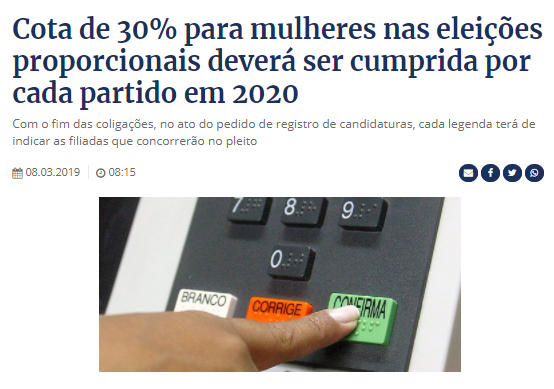
\includegraphics[width=.75\linewidth]{cotafe.png}

\end{figure}


Pensando na importância da representatividade feminina para além das questões políticas e considerando uma turma de 22 estudantes mulheres e 18 estudantes homens responda os questionamentos abaixo. 
 
\begin{enumerate}
\item Quantas comissões de 6 estudantes é possível formar, mantendo exatamente o mínimo de representação feminina?

\textit{Solução do grupo:}  

\begin{enumerate}[label=\titem{\arabic*.}]
\item Para manter exatamente o mínimo de representação feminina a equipe deve ter exatamente 2 mulheres.
\item Usando o princípio multiplicativo e considerando o número de mulheres e homens; e depois levando em conta que não importa a ordem de escolha, dividimos por $6!$ para retirar as repetições. Obtendo
$$\dfrac{22\cdot 21\cdot 18 \cdot 17 \cdot 16 \cdot 15}{6!} = 47.124,$$
que seria o número de comissões possíveis com 2 mulheres e 4 homens. 
\end{enumerate}



\item Quantas comissões de 6 estudantes é possível formar, mantendo as regras de representatividade determinadas pelo TSE?


\textit{Solução do grupo:}

\begin{enumerate}[label=\titem{\arabic*.}]
\item Para manter a regra devemos ter no mínimo duas mulheres. 
\item Basta escolhermos primeiro duas mulheres, isso pode ser feito de $\dfrac{22 \cdot 21}{2!}$.
\item Para as outras 4 pessoas restantes, que podem ser homens ou mulheres, pegamos o total de pessoas que sobraram $20+18=38$ e delas escolhemos 4:
$\dfrac{38 \cdot 37\cdot 36 \cdot 35}{4!}$ maneiras de fazer essa escolha. 
\item Usando o Princípio Multiplicativo, $\dfrac{22 \cdot 21}{2!} \cdot \dfrac{38 \cdot 37 \cdot36 \cdot 35}{4!}= 17.051.265$ comissões.
\end{enumerate}

\item Se Eduardo e Lucas são dois colegas de turma que não conseguem trabalhar juntos em equipe. Quantas seriam as comissões possíveis considerando mais esta restrição? 


\textit{Solução do grupo:}

\begin{enumerate}[label=\titem{\arabic*.}]
\item Como o cálculo do número de comissões já foi feito nos itens anteriores decidimos retirar deste total as comissões que estão Eduardo e Lucas juntos. Basta então contar as possibilidades de escolha de 4 pessoas de um total de 38, já que Eduardo e Lucas já foram escolhidos. Isso pode ser feito de $\dfrac{38 \cdot 37 \cdot 36 \cdot 35}{4!} = 73.815.$ maneiras. Total de comissões em que Eduardo e Lucas não estão juntos é dado por $17051265-73.815=169777450.$
\end{enumerate}
\end{enumerate}

\end{task}

\begin{task}{Produzindo Acessórios}

Para a produção de algumas bijuterias, como brincos e braceletes são usadas pedras de três cores diferentes. Levando em conta três cores, responda:
 
\begin{enumerate}
\item O modelo dos brincos é dado por um quadrado com uma pedra em cada um dos vértices e com o fecho na parte de trás de uma das pedras. 

\begin{figure}[H]
\centering

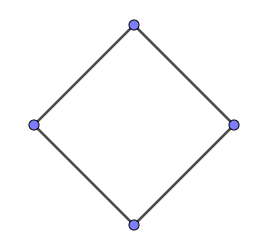
\includegraphics[scale=0.4]{brincos.png}
\end{figure}

Pense em alguns modelos de brinco que usem exatamente as  três cores de pedras disponíveis de modo que duas pedras na sequência não sejam da mesma cor.

\item A turma conseguiu muitos modelos diferentes? Compare seu modelo com o dos amigos.
\item Quantos brincos diferentes é possível produzir levando em conta a restrição das cores dada no item a)?
\item O modelo dos braceletes é dado por 4 peças contendo uma pedra cada igualmente espaçadas.  Quantos braceletes é possível fabricar levando em conta a mesma restrição nas cores?
\item Quantos conjuntos diferentes com um par de brincos e um bracelete é possível formar? Eles não precisam necessariamente ter a mesma organização nas cores.
\item Pensando em outro modelo de brinco, formado por 8 pequenos pêndulos com uma pedra em cada, não faz mais sentido pensar na restrição para as cores lado a lado. O que diferencia uma bijuteria da outra agora é a quantidade de pedras de uma determinada cor. Supondo ainda que temos que ter pedras das três cores disponíveis,  quantas peças diferentes deste tipo é possível produzir?  
\item E se na produção dos brincos em pêndulos fosse permitido agora ter até 3 cores e não mais exatamente 3 cores? 
      
 \end{enumerate}
\end{task}

\arrange{Contando agrupamentos}

Voltemos ao questionamento proposto no início da seção. O número de maneiras de se retirar 3 bolas amarelas e 2 vermelhas de uma urna com 5 bolas, sem reposição, tem alguma relação com o número de maneiras de se escolher 3 pessoas de um grupo de 5? Apesar de serem agrupamentos diferentes:  o primeiro temos um agrupamento de 5 bolas com repetição das bolas amarelas (aparecem 3 vezes) e repetição das bolas vermelhas (aparecem 2 vezes); já o segundo é um conjunto de 3 pessoas escolhidas dentre 5 pessoas distintas, a solução de ambos os problemas é a mesma, $\dfrac{5!}{2!3!}.$
Assim, é difícil caracterizar todos os problemas e tipos de agrupamentos existentes por meio de suas soluções. Não existe um passo a passo pré-definido para a resolução de todos os problemas de contagem, cada um deve ser lido, interpretado e os passos construídos de maneira específica, é preciso se imaginar resolvendo o problema. Os cálculos seguem a mesma linha dos passos organizados, cada etapa definida corresponde a uma parte da solução.  Ao pensar na solução para um problema de contagem alguns questionamentos devem ser feitos:

\begin{enumerate}

    \item O problema tem algum tipo de restrição?
    
    As restrições devem ser consideradas primeiro, caso isso não seja feito pode ser que sua solução fique muito complicada.

    \item É preciso quebrar o problema em casos mais simples?
    
    Alguns problemas parecem muito difíceis a primeira vista, mas quando interpretados com cuidado podem ser divididos em casos menores cuja resolução seja mais simples. (\textbf{Princípio Aditivo})
    
    \item O referencial escolhido está correto?
    
    Os problemas podem ser resolvidos por diferentes caminhos, tomando diferentes referenciais para contagem. Algumas escolhas deixam o problema mais difícil por conta do número de casos a se considerar. 
    
    \item Os elementos que compõe a contagem fazem parte de conjuntos disjuntos (conjuntos que não possuem elementos comuns)?
    
    Se o \textbf{Princípio Multiplicativo} é usado para contagem de sucessivos elementos tomados em conjuntos disjuntos ele não impõe ordem. Caso contrário, se o agrupamento for tomado no mesmo conjunto, sua utilização impõe ordem. 
    
    \item Os objetos contados são distintos? 
    
    Existe a possibilidade de ter disponível várias cópias do mesmo objeto para a composição dos agrupamentos.
    
    \item A repetição dos elementos na contagem é permitida?
    
    O problema pode descrever elementos distintos, mas que podem ser repetidos.

    \item Todos os elementos disponíveis precisam ser usados?
    
    Alguns agrupamentos usam todos os elementos do conjunto outros usam parte deles. 
    
    \item A estratégia escolhida realmente conta cada um dos casos uma única vez? 
    
    Depois de pensar no caminho para a solução é preciso refletir se realmente todos os elementos de interesse foram contados uma única vez. Essa mesma reflexão pode ser feita a fim de verificar se existem elementos contados a mais ou a menos.
    
\end{enumerate}

\practice{Contando Agrupamentos}

\begin{task}{Hora de criar}
Nas Atividades desenvolvidas foi possível perceber a variedade de situações e técnicas de resolução de problemas de contagem. Agora é a hora de criar os seus problemas. Vocês podem manter todos os problemas em torno de uma única temática ou variar os assuntos abordados. Mãos à obra!

\begin{enumerate}

    \item Crie um problema de contagem que envolva dois conjuntos disjuntos; 
    \item Crie um problema de contagem no qual a ordem dos elementos no agrupamento não seja importante;
    \item Crie um problema de contagem que envolva organizar elementos em roda;
    \item Crie um problema de contagem em que todos os itens anteriores sejam satisfeitos. 
    \item Agora resolva os problemas criados por outros grupos. As ideias foram parecidas?
    
\end{enumerate}
\end{task}

\know{Generalizando}

\paragraph{Para que servem as calculadoras?}

\begin{center}
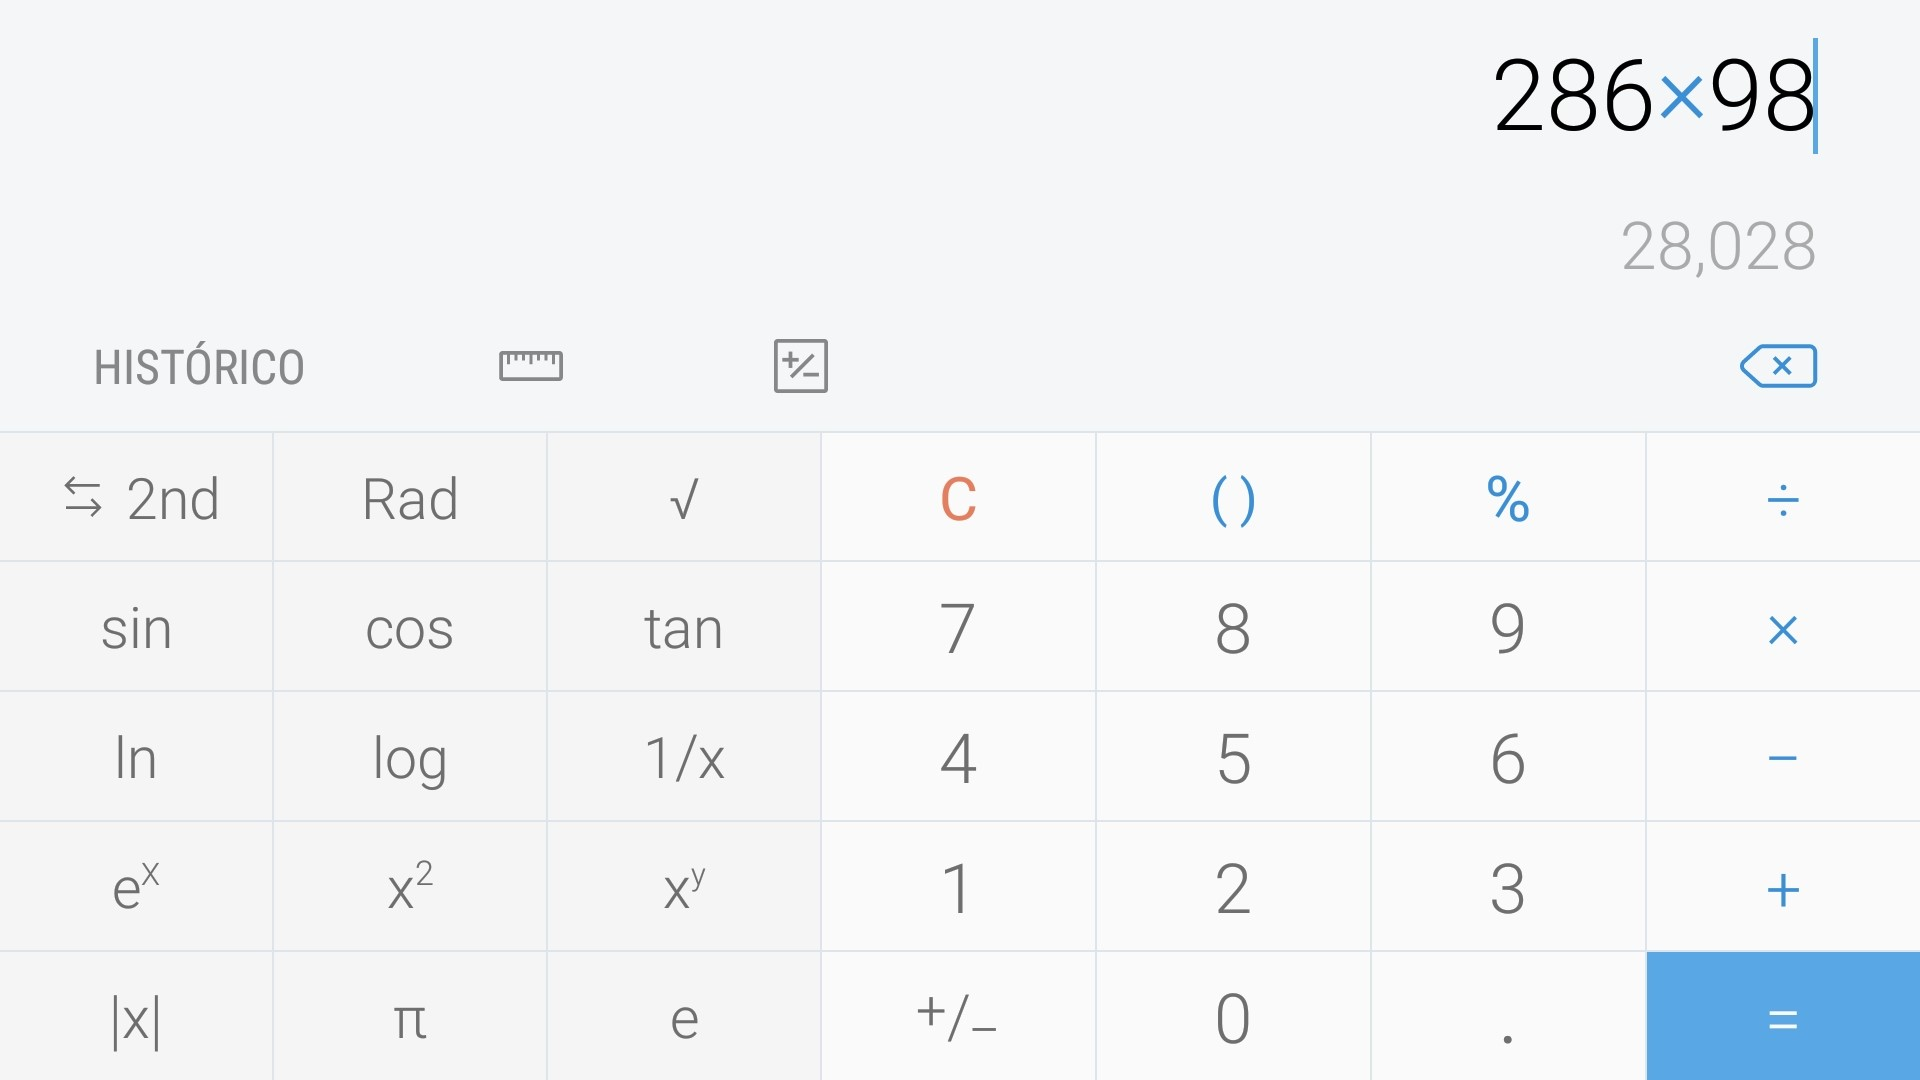
\includegraphics[scale=0.18]{calculadora.jpeg}
\end{center}

Vocês já pararam para pensar no surgimento da primeira calculadora? 
Hoje existem no mercado vários tipos delas, online ou não, desde as mais simples até as mais sofisticadas. Estão presentes até nos aparelhos celulares. Pra que elas servem? Elas ajudariam a solucionar os problemas pensados neste livro?

\begin{task}{Calculadora Combinatória}
Uma calculadora não é capaz de resolver os problemas do cotidiano, mas ela pode diminuir e muito o tempo de realização dos cálculos. Sabendo como usar, ela é uma forte aliada nas tarefas do dia a dia. Projete com seus colegas de grupo uma Calculadora Combinatória.



Os agrupamentos mais comuns estão descritos abaixo, mas o grupo pode pensar outras organizações possíveis e úteis de acordo com sua percepção dos problemas estudados no material.

\begin{itemize}
\item \textbf{Arranjo:}  é uma maneira de organizar em fila parte dos elementos de um determinado conjunto de elementos distintos. Considerando o conjunto $\{1,2,3,4,5\}$, o número 253 é um arranjo formado por três elementos deste conjunto com cinco elementos, que é diferente do arranjo 532. Neste caso os arranjos são diferentes e a ordem em que os elementos estão organizados é importante, trocar a ordem de elementos significa gerar outro arranjo com os mesmos elementos. A notação para o número de arranjos possíveis com $p$ elementos de um conjunto com $n$ elementos distintos é  dada por $A_n^p$ ou  $A_{n,p},$ 


\item \textbf{Permutação:} é um embaralhamento de elementos distintos. Leva em conta elementos distintos e se refere a organização deles em fila. Pode ser considerado um arranjo de todos os elementos do conjunto. Comumente usa-se a notação $P_n$ para o número de permutações de $n$ objetos. 


\item \textbf{Combinação:} é um subconjunto de um conjunto de elementos distintos. Ou ainda, um agrupamento formado pela escolha de elementos de um conjunto dado. Por exemplo, considerando o conjunto $\{1,2,3,4,5\}$, uma combinação formada por três elementos dele é dada por $\{2,5,3\}$. A ordem da escolha não interfere no subconjunto criado, apenas leva em conta que os elementos são distintos.  Notação normalmente usada $C_n^p,C_p^n$ ou ainda, $C_{n,p}$ para o número de combinações possíveis com $p$ elementos de um conjunto com $n$ elementos. 


\item \textbf{Agrupamento com repetição:} é um agrupamento tomado em um conjunto que possua várias cópias de determinados objetos, ou que um mesmo elemento possa ser usado mais de uma vez. Exemplos: 121 é um tipo de arranjo dos algarismos que permite a repetição.  Escolher duas bolas vermelhas e uma azul de uma urna contendo 3 bolas vermelhas, 4 bolas azuis e 2 amarelas é um agrupamento com objetos repetidos. É possível considerar permutação, arranjo e combinação com repetição. 
\end{itemize}


\begin{enumerate}
\item Quais botões a calculadora precisa ter para resolver os problemas os problemas de contagem estudados aqui? 

\item Quais botões podem ser incluídos a calculadora para incluir a contagem dos agrupamentos comuns estudados aqui? Como incluir a possibilidade de repetição de objetos?


\item Faça um desenho que represente a calculadora e explique a funcionalidade de cada um dos botões.

\end{enumerate}
\end{task}

\begin{task}{Testando a calculadora combinatória}
Nos problemas a seguir escreva uma solução e descreva a sequência de botões, na sua calculadora, que seria necessária para encontrar a solução correta.

\begin{enumerate}
\item (Enem 2016, adaptada) O tênis é um esporte em que a estratégia de jogo a ser adotada depende, entre outros fatores, de um adversário ser canhoto (joga usando a mão esquerda) ou destro (joga usando a mão direita). 

Um clube tem um grupo de 10 tenistas, sendo que 4 são canhotos e 6 são destros. O técnico do clube deseja realizar uma partida de exibição entre dois desses jogadores, porém não poderão ser ambos canhotos. Qual o número de possibilidades de escolha dos tenistas para a partida de exibição.  

\item (Enem 2016, adaptada) Para cadastrar-se em um \textit{site}, uma pessoa precisa escolher uma senha composta por quatro caracteres, sendo dois algarismos e duas letras (maiúsculas ou minúsculas). As letras e algarismos podem estar em qualquer posição. Essa pessoa sabe que o alfabeto é composto por vinte e seis letras e que uma letra maiúscula difere da minúscula em uma senha. 
 {Disponível em: www.infowester. com. Acesso em 14 dez. 2012.}
 
Qual o número total de senhas possíveis para o cadastramento nesse site?

\item Em uma escola de música, 7 professores tocam algum instrumento e outros 3 cantam. Ocorrerá uma festa onde 4 dos 10 serão contratados, com pelo menos 1 que cante. Quantas equipes podem ser formadas?

\end{enumerate}
\end{task}

Algumas características de problemas combinatórios são comuns, o que torna possível organizá-los em alguns tipos de agrupamentos: arranjos, permutações e combinações, com ou sem repetições. As fórmulas nada mais são do que o resumo da contagem para cada tipo de agrupamento. Mas saber apenas as fórmulas não significa conseguir resolver um problema de contagem. As ideias trabalhadas neste material seguiram no sentido de discutir algumas possibilidades de solução e apresentar maneiras de organização do raciocínio, mas para resolver um problema de contagem é necessário realmente traçar um passo a passo de ações que podem ser traduzidas em operações matemáticas.
Os verbos que mais aparecem são  escolher, permutar e arranjar, mais fortemente escolher e permutar. 

Escolher se refere ao ato de tomar um subconjunto de um conjunto dado, neste ato não importa em que ordem essa escolha foi feita, importa apenas quais elementos foram escolhidos. Permutar é equivalente ao ato de  embaralhar ou enfileirar os elementos. Arranjar por outro lado se refere a um embaralhamento de elementos escolhidos, ou de embaralhamento de parte dos elementos de um conjunto. Escolher e depois embaralhar é equivalente a arranjar. Assim, o número de arranjos de $p$ elementos dentre $n$ elementos distintos é calculado se escolhermos $p$ dentre $n$ elementos possíveis, e depois multiplicar esse valor pela permutação desses $p$ elementos. 

Na linguagem matemática podemos escrever

\begin{align*}
A_n^p&= p! \cdot C_n^p,\\
C_n^p&= \dfrac{A_n^p}{p!}.
\end{align*}

Mais do que fórmula, é importante reconhecer os usos do Princípio Aditivo e Multiplicativo. Resolver um problema combinatório é realizar uma sequência de passos que leva em conta esses três atos: escolher, permutar (ou embaralhar) e arranjar, combinados com as operações básicas.



\exercise

\begin{enumerate}
\item  Quantas são as diferentes possibilidades de organizar o nome de uma equipe com as iniciais B, A, L, I, E, K? De quantas maneiras diferentes 6 pessoas podem ser organizadas em fila? Qual o número de permutações dos números $9, 5, 8, 2, 4, 1?$

\item Quantas seriam as diferentes possibilidades de formar o nome de uma equipe com as inicias de seus membros, sendo eles: Fabrício, Bruna, Bianca e Fábio? 

\item Em uma turma composta por 40 alunos será realizada uma gincana e para isso eles serão dividimos em 5 equipes. A equipe amarela será a primeira a ser formada. De quantas maneiras diferentes esta equipe pode ser formada?

\item Suponha que para montar os uniformes para um jogo de futebol a escola tenha camisetas de três cores diferentes: amarela, branca e vermelha. E possua quatro tipos de bermudas: amarela, azul, preta e cinza. Seria bem estranho vestir o time todo de amarelo, camiseta e bermuda. Levando isso em conta, quantos uniformes diferentes poderiam ser criados?

\item Para realização das atividades a professora de uma turma com 40 alunos quer organizar os grupos sorteando seus membros. Para isso possui 8 fitas de cada uma das seguintes cores: amarela, vermelha, laranja, branca e preta. Essas fitas serão escolhidas de maneria aleatória sendo misturadas em um recipiente que não seja possível verificar a cor da fita até que seja totalmente retirada.  Joana, uma aluna desta turma, tem uma amiga muito querida e está torcendo para que fiquem no mesmo grupo. Será que as chances disso acontecer são grandes ou pequenas?

\item Qual o número de permutações de um conjunto com 40 objetos, os quais são organizados em 5 tipos diferentes, cada tipo contendo 8 objetos? Este problema pode ser relacionado com o problema anterior de alguma maneira?

\item Se ao invés de 5 grupos de $8$ elementos, tivéssemos o total de 8 grupos de $5$ elementos. O número de maneiras diferentes de organizar as equipes seria maior ou menor? 

\item Uma empresa confecciona e comercializa um brinquedo formado por uma locomotiva pintada na cor preta, mais 12 vagões de iguais formato e tamanho, numerados de 1 a 12. Dos 12 vagões, 4 são pintados de cor vermelha, 3 na cor azul, 3 na cor verde, e 2 na cor amarela. O trem é montado utilizando-se uma locomotiva e 12 vagões, ordenados crescentemente segundo suas numerações, conforme ilustrado na figura: 

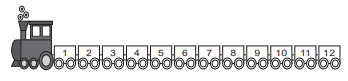
\includegraphics[scale=1]{exe1}

De acordo com as possíveis variações nas colorações dos vagões, a quantidade de trens que pode ser montados, expressa por meio de combinações, é dada por: 

\begin{enumerate}
\item $C^4_{12} \times C^3_{12} \times C^3_{12} \times C^2_{12}$
\item $C^4_{12} + C^3_{8} + C^3_{5} + C^2_{2}$
\item $C^4_{12} \times 2 \times C^3_{8} \times C^2_{5}$
\item $C^4_{12} + 2 \times C^3_{12} \times C^2_{12}$
\item $C^4_{12} \times C^3_{8} \times C^3_{5} \times C^2_{2}$
\end{enumerate}


\item O Salão do Automóvel de São Paulo é um evento no qual vários fabricantes expõe seus modelos mais recentes de veículos, mostrando, principalmente, suas inovações em \textit{design} e tecnologia. 
\begin{flushright}
\small{disponível em http: //g1.globo.com. Acesso em: 4 fev. 2015 (adaptado)}
\end{flushright}

Uma montadora pretende participar desse evento com dois estandes, um na entrada e o outro na região central do salão, expondo, em cada um deles, um carro compacto e uma caminhonete.
Para compor os estandes, foram disponibilizados pela montadora quatro carros compactos, de modelos distintos, e seis caminhonetes de diferentes cores para serem escolhidos aqueles que serão expostos. A posição dos carros dentro de cada estande é irrelevante.
Uma expressão que fornece a quantidade de maneiras diferentes que os estandes podem ser compostos é
 
 \begin{enumerate}
\item $A^4_{10}$
\item $C^4_{10}$
\item $C^2_{4} \times  C^2_{6} \times 2 \times 2$
\item $A^2_{4} \times A^2_{6} \times 2 \times 2$
\item $C^2_{4} \times C^2_{6}$
\end{enumerate}

\item Um brinquedo infantil caminhão-cegonha é formado por uma carreta e dez carrinhos nela transportados, conforme a figura:


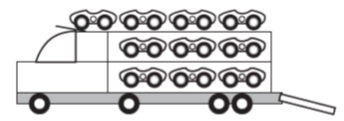
\includegraphics[scale=1]{exe2}

No setor de produção da empresa que fabrica esse brinquedo, é feita a pintura de todos os carrinhos para que o aspecto do brinquedo fique mais atraente. São utilizadas as cores amarelo, branco, laranja e verde, e cada carrinho é pintado apenas com uma cor. O caminhão-cegonha tem uma cor fixa. A empresa determinou que em todo caminhão-cegonha deve haver pelo menos um carrinho de cada uma das quatro cores disponíveis. Mudança de posição dos carrinhos no caminhão cegonha não gera um novo modelo do brinquedo.
Com base nessas informações, quantos são os modelos distintos do brinquedo caminhão-cegonha que essa empresa poderá produzir?
 
 \begin{itemize}
 
\item $C_{6,2}$
\item $C_{9,3}$
\item $C_{10,4}$
\item $6^4$
\item $4^6$
\end{itemize}

\item (Unesp 2016) Está previsto que, a partir de $1^{o}$ de janeiro de 2017, entrará em vigor um sistema único de emplacamento de veículos para todo o Mercosul, o que inclui o Brasil. As novas placas serão compostas por 4 letras e 3 algarismos. Admita que no novo sistema possam ser usadas todas as 26 letras do alfabeto, incluindo repetições, e os 10 algarismos, também incluindo repetições. Admita ainda que, no novo sistema, cada carro do Mercosul tenha uma sequência diferente de letras e algarismos em qualquer ordem. Veja alguns exemplos das novas placas.

\begin{center}
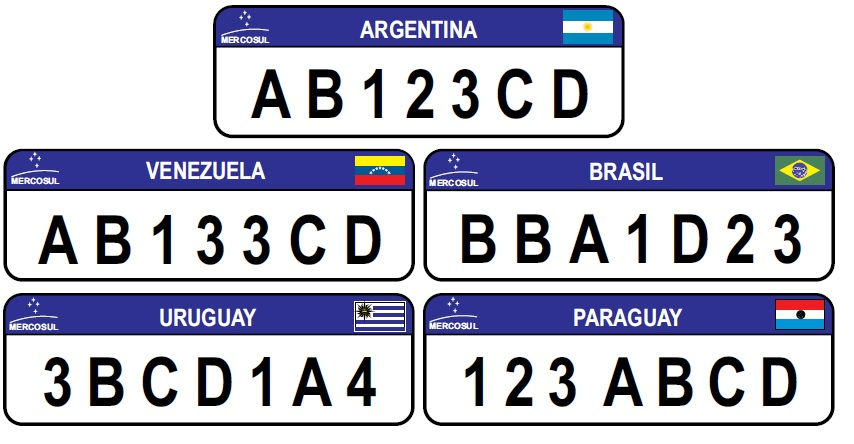
\includegraphics[scale= 0.4]{2f_2016_fig1.jpg}
\end{center}

Imagem: \url{https://drive.google.com/file/d/0Bz49JztKIEhLYmpoVXB6QklMaXc/view}

No novo sistema descrito, calcule o total de placas possíveis com o formato “Letra-Letra-Algarismo-Algarismo–Algarismo-Letra-Letra”, nessa ordem. Em seguida, calcule o total geral de possibilidades de placas com 4 letras (incluindo repetição) e 3 algarismos (incluindo repetição) em qualquer ordem na placa. Deixe suas respostas finais em notação de produto ou de fatorial.

\item Em Hogwarts, uma escola de magia e bruxaria dos filmes e livros de Harry Potter, todos os anos 16 alunos bruxos são divididos em 4 casas, 4 em cada casa, sendo elas: Grifinória, Sonserina, Corvinal e Lufa-Lufa. O personagem principal Harry se torna muito amigo de Rony e os mesmos querem ficar na mesma casa.  Considerando todas as possíveis divisões destes bruxos nas casas, quantas são as chances de Harry e Rony ficarem juntos?

 \item Em Hogwarts, uma escola de magia e bruxaria dos filmes e livros de Harry Potter, todos os anos 16 alunos bruxos são divididos em 4 casas, 4 em cada casa, sendo elas: Grifinória, Sonserina, Corvinal e Lufa-Lufa. O personagem principal Harry não gostaria de estar na mesma casa que  Draco Malfoy. Considerando todas as possíveis divisões destes bruxos nas casas, quantas são as chances de Harry e Malfoy ficarem separados?
\end{enumerate}

\ifnum\aluno=1
\clearpage
\else
\notasfinais
\fi

\bibliographystyle{apalike-pt}
\bibliography{../Bibliografia/combinatoria_bibliografia.bib}

\nocite{*}